\chapter{Proposed Method}
\label{ch:method}

This chapter presents HSGE (Hierarchical Skill-Graph Exploration), our
pipeline for turning an unannotated website into training data for a small
language model. The chapter covers (1) an overview of the pipeline and its
design principles, (2) the two-level graph representation that underlies it,
(3) graph-guided exploration with LLM-proposed low-level tasks, (4) the
discovery and verification of reusable skills, (5) the generation of
long-horizon \emph{semantic tasks} by chaining planning operators, (6) the
curation of collected trajectories into a fine-tuning dataset, (7) the
fine-tuning of the target SLM, and (8) implementation notes.

\section{Overview}
\label{sec:method-overview}

The input to HSGE is a live website with no task annotations, together with a
frontier of one or more seed URLs. The output is a supervised fine-tuning
(SFT) dataset of goal-conditioned interaction trajectories, and ultimately a
small language model fine-tuned on that dataset. Figure~\ref{fig:pipeline}
shows the overall architecture.

\begin{figure}[htbp]
\centering
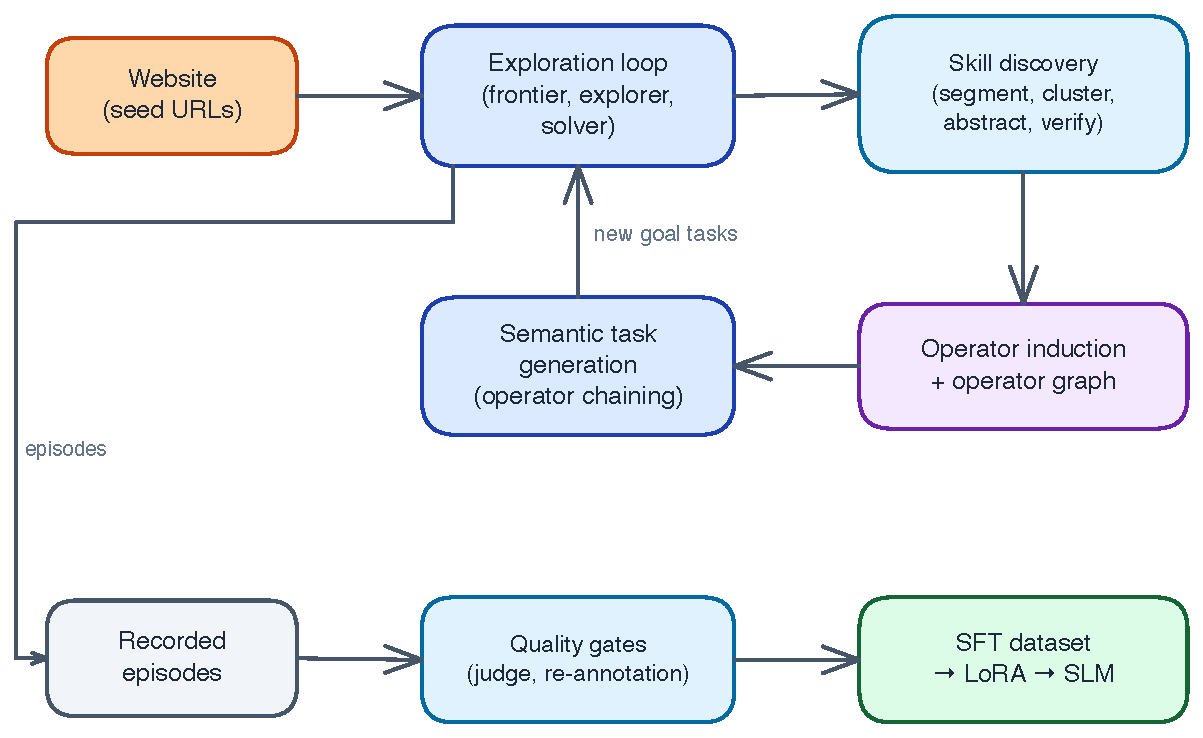
\includegraphics[width=\textwidth]{Figures/fig_pipeline.pdf}
\caption[Overview of the HSGE pipeline]{Overview of the HSGE pipeline. The
exploration loop solves LLM-proposed low-level tasks on frontier pages;
discovered skills are lifted into planning operators, whose chains are fed
back into the loop as semantic tasks. All recorded episodes pass through
quality gates before becoming fine-tuning data.}
\label{fig:pipeline}
\end{figure}

The pipeline operates as a loop. An \emph{explorer} proposes concrete,
page-grounded tasks on each visited page, and a \emph{solver} agent attempts
them in a real browser, producing interaction trajectories. A discovery
component segments these trajectories, clusters recurring segments, abstracts
each mature cluster into a reusable \emph{skill}, and lifts verified skills
into planning \emph{operators} with explicit preconditions and effects.
Chaining operators over the resulting graph yields composed, long-horizon
goal tasks --- the \emph{semantic tasks} --- which are fed back into the same
solver, closing the loop. Every attempted task, whether low-level or
semantic, is recorded as an episode; episodes then pass through automated
quality gates and are compiled into the SFT dataset used to fine-tune the
target SLM.

Three design principles run through the pipeline:

\begin{itemize}
  \item \textbf{P1 --- Verify before reuse.} Nothing is trusted on first
  sight. A skill is admitted only after it has recurred across independent
  trajectories; a declared task success is re-checked by an independent
  judge; an induced operator is rejected if its effects are vacuous.
  \item \textbf{P2 --- Graph over flat.} Instead of a flat pool of pages or
  memories, HSGE maintains a two-level graph (Section~\ref{sec:method-graph}).
  The low level records where the agent has been; the high level records what
  the agent can \emph{do}, and how those capabilities connect.
  \item \textbf{P3 --- A two-tier task hierarchy.} LLM-proposed
  \emph{low-level tasks} (Section~\ref{sec:method-exploration}) drive
  exploration and supply the raw material for skill discovery. \emph{Semantic
  tasks} (Section~\ref{sec:method-semantic}) are generated only from the
  operator graph, by composing verified capabilities into goals that no
  single page suggests.
\end{itemize}

\section{Two-Level Graph Representation}
\label{sec:method-graph}

\begin{figure}[htbp]
\centering
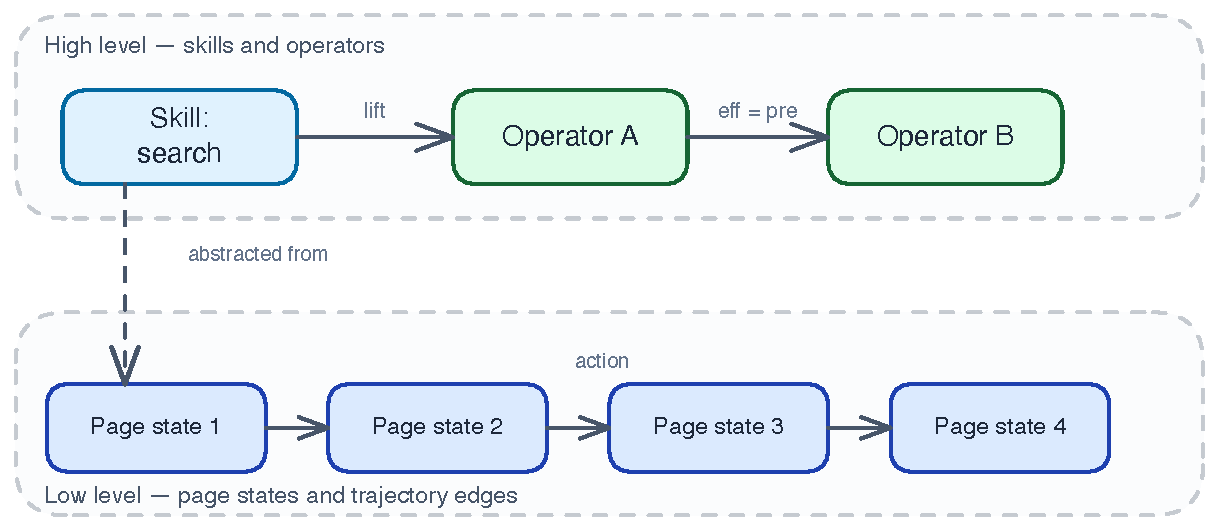
\includegraphics[width=0.95\textwidth]{Figures/fig_twolevel.pdf}
\caption[The two-level graph]{The two-level graph. The low level records
visited page states and the trajectory edges (actions) between them; the high
level records skills, lifted into planning operators and wired by composition
edges where one operator's effect matches the next one's precondition. Skills
are grounded in the low level through abstraction and initiation/effect
links.}
\label{fig:twolevel}
\end{figure}

\subsection{The website as a decision process}

We model the website as a partially observable decision process. At each step
the agent observes $o = (u, x)$, where $u$ is the current URL and $x$ is the
\emph{accessibility tree} (axtree) of the page: a text serialization of the
visible interface elements, each carrying a stable element identifier. The
agent acts through a fixed action space $\mathcal{A}$
(Table~\ref{tab:actions}), which covers element interaction, navigation, tab
management, and two terminal actions that end an episode: answering the user
and declaring the task infeasible. A \emph{trajectory} is the sequence
$\tau = \langle (o_0, a_0), (o_1, a_1), \dots \rangle$ produced while
attempting one task.

\begin{table}[H]
\centering
\caption[The solver's action space]{The solver's action space. Element
arguments refer to identifiers shown in the accessibility tree.}
\label{tab:actions}
\small
\begin{tabular}{L{5.4cm} L{7.8cm}}
\toprule
\textbf{Action} & \textbf{Meaning} \\
\midrule
\texttt{click(id)} & Click the element \texttt{id}. \\
\texttt{fill(id, text)} & Type \texttt{text} into the field \texttt{id}. \\
\texttt{select\_option(id, opt)} & Choose \texttt{opt} in the dropdown \texttt{id}. \\
\texttt{press(id, key)} & Send a keyboard shortcut to \texttt{id}. \\
\texttt{goto(url)}, \texttt{go\_back()} & Navigate directly / go back in history. \\
\texttt{new\_tab()}, \texttt{tab\_focus(i)}, \texttt{tab\_close()} & Tab management. \\
\texttt{send\_msg\_to\_user(text)} & Terminal: report the answer or completion. \\
\texttt{report\_infeasible(reason)} & Terminal: declare the task impossible. \\
\bottomrule
\end{tabular}
\end{table}

\subsection{Low level: page states and trajectory edges}

The low level of the graph records concrete experience: nodes are visited
page states, identified by URL and by a hash of the initial axtree, and edges
are the actions the agent actually executed between them. Hashing page
content, rather than trusting URLs alone, matters in practice: two distinct
URLs frequently render the same page, and revisiting them would waste an
entire exploration budget on content the agent has already seen.

\subsection{High level: skills as options}

A \emph{skill} is a reusable, parameterized capability, formalized in the
options framework~\cite{sutton1999options} as a triple
$\sigma = \langle I, \pi, \beta \rangle$: an initiation set $I$ (page states
where the skill applies), a policy $\pi$ (the action procedure), and a
termination condition $\beta$. Concretely, HSGE represents a skill as a
\emph{skill card}: a name, a natural-language description, a list of typed
parameter slots (for example a search query or a form value), and links to
the member trajectory segments it was abstracted from. Skill nodes are wired
to low-level states by initiation and effect edges, and to each other by
composition edges, forming the high-level graph.

\subsection{Operators: preconditions and effects}

Planning over raw skills is difficult because their applicability is
implicit. HSGE therefore lifts each verified skill into an
\emph{operator} in the classical STRIPS style~\cite{fikes1971strips}:
$\omega = \langle \mathit{pre}, \mathit{eff} \rangle$, where $\mathit{pre}$
and $\mathit{eff}$ are sets of natural-language predicates such as ``user is
viewing a project's issue list''. Unlike classical planning, the predicate
vocabulary is not fixed in advance: predicates are authored freely by an LLM
during induction and then \emph{canonicalized} into stable identifiers by an
embedding-based clusterer (Section~\ref{sec:method-semantic}), so that two
paraphrases of the same condition resolve to the same predicate. The
\emph{operator graph} draws an edge from operator $\omega_1$ to $\omega_2$
whenever an effect of $\omega_1$ satisfies a precondition of $\omega_2$;
paths in this graph are executable multi-skill plans.

\subsection{Task terminology}

Throughout this thesis we distinguish two tiers of tasks. A \emph{low-level
task} is a short, page-grounded instruction proposed by the explorer while
visiting a page (for example, ``open the most recently updated merge
request''). A \emph{semantic task} is a long-horizon goal generated from the
operator graph by chaining at least two operators; it exists only because the
graph exists, and it is the central product of the method.

\section{Graph-Guided Exploration}
\label{sec:method-exploration}

Exploration must answer three questions at every step: \emph{where} to go
next, \emph{what} to try there, and \emph{how} to try it. HSGE assigns these
to the frontier, the explorer, and the solver, respectively.

\subsection{Frontier management}
\label{sec:method-frontier}

The frontier is a priority queue over candidate URLs with two tiers of
candidates. \emph{Tier~0} contains URLs the agent actually reached while
solving tasks, together with pages left open in browser tabs; these are
admitted directly, subject only to allow/deny and visited checks, because
reaching them is itself evidence that they matter. \emph{Tier~1} contains
hyperlinks mined from each visited page's DOM. Mining hyperlinks is
essential: growth would otherwise depend entirely on task-driven navigation,
and a page whose tasks are all informational would contribute nothing to the
frontier --- a failure mode we return to in Chapter~\ref{ch:discussion}.

Mined links, however, arrive in bulk and are dominated by near-duplicates
(every post, comment, and user profile of a forum shares one page shape). To
keep them from flooding the queue, each URL is normalized into a
\emph{URL template}: the scheme, query, and fragment are dropped, and
identifier-like path segments --- together with everything after them --- are
replaced by wildcards, so that
\begin{center}
\texttt{/f/AskReddit/comments/12345/title}
$\;\rightarrow\;$
\texttt{/f/AskReddit/comments/*/*}.
\end{center}
At most $c$ pages per template are
visited (default $c = 3$), and the cap is re-checked lazily when a candidate
is popped, since a template's visit count grows during the run. Within
tier~1, candidates from unseen templates are preferred, then shallower pages,
then insertion order. Algorithm~\ref{alg:frontier} summarizes the loop; a
node whose initial page content hashes identically to an already-visited node
is skipped outright.

\begin{algorithm}[H]
\caption{Graph-guided exploration loop}
\label{alg:frontier}
\begin{algorithmic}[1]
\State $F \gets$ priority queue seeded with start URLs; $V \gets \emptyset$
\While{$F \neq \emptyset$ \textbf{and} node budget remains}
  \State $u \gets \textsc{Pop}(F)$ \Comment{key: (tier, template novelty, depth, seq)}
  \If{template cap of $u$ exhausted \textbf{or} $\textsc{Hash}(u) \in V$} \textbf{continue} \EndIf
  \State $V \gets V \cup \{\textsc{Hash}(u)\}$
  \State $T \gets \textsc{Explorer}(u)$ \Comment{low-level tasks, Sec.~\ref{sec:method-lowlevel}}
  \State $T \gets T \cup \textsc{SemanticTasks}()$ \Comment{operator chains, Sec.~\ref{sec:method-semantic}}
  \For{task $t \in T$}
    \State $\tau \gets \textsc{Solver}(u, t)$; record episode; $\textsc{Discovery}(\tau)$
    \State add URLs reached in $\tau$ to $F$ as tier~0
  \EndFor
  \State mine hyperlinks of $u$; add as tier~1 under template caps
\EndWhile
\end{algorithmic}
\end{algorithm}

\subsection{Low-level task proposal}
\label{sec:method-lowlevel}

On each frontier page, an LLM-based \emph{explorer} proposes up to $k$
concrete tasks (default $k = 6$) grounded in the page content. Each proposal
is returned in a structured form with an explicit type field ---
\texttt{INFO} (information seeking), \texttt{NAV} (navigation), or
\texttt{MOD} (state modification) --- rather than as free text with an
embedded tag, which production runs showed models do not reliably emit. The
classification is load-bearing: in a \emph{read-only} mode used on shared
sites, \texttt{MOD} tasks and any task the model failed to classify are
dropped fail-closed, since an unclassifiable task might be a modification in
disguise.

Two mechanisms keep proposals diverse. First, the explorer persists for the
whole run and remembers every task text it has already proposed; recent
proposals are echoed back into the prompt as negative context, and near
duplicates are additionally dropped in code. Without this, a large fraction
of proposals degenerate into sitewide navigation boilerplate repeated on
every page. Second, when the proposal list must be truncated to $k$,
information-seeking tasks are cut first: solving an \texttt{INFO} task never
navigates anywhere, so it can never grow the frontier.

These proposals are deliberately \emph{low-level}: each is scoped to what a
single page affords. Their role is to generate diverse, realistic
trajectories --- the raw material from which skills, and eventually semantic
tasks, are derived.

\subsection{The task solver}
\label{sec:method-solver}

\begin{figure}[htbp]
\centering
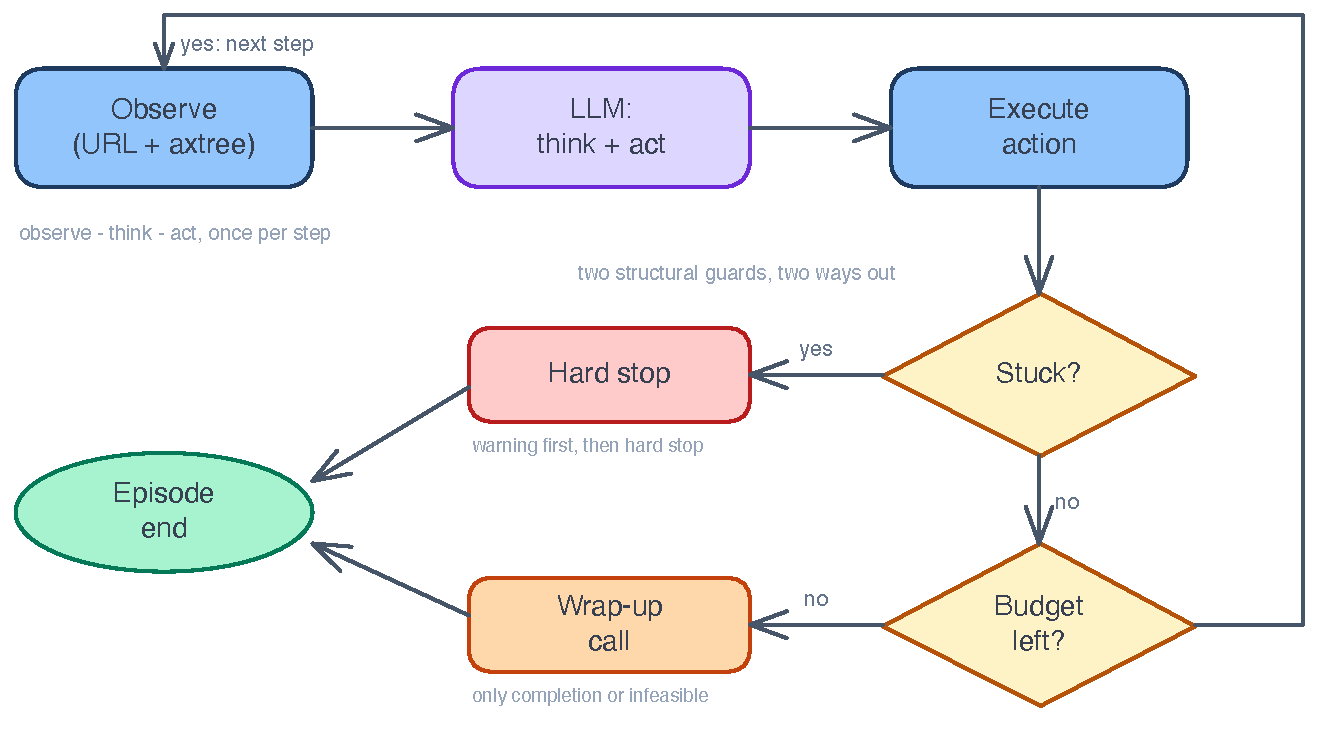
\includegraphics[width=\textwidth]{Figures/fig_solver.pdf}
\caption[The solver loop with structural guards]{The solver's
observe--think--act loop. A stuck-loop guard hard-stops the episode when
actions repeat on the same target with no observable change; an exhausted
step budget triggers a single wrap-up call that may only declare success or
infeasibility.}
\label{fig:solver}
\end{figure}

The \emph{solver} is a ReAct-style agent loop~\cite{yao2023react}: at each
step it receives the goal, the current URL, the (length-capped) accessibility
tree, and a window of its recent actions, each annotated with its observed
outcome (``now at $\langle$url$\rangle$'', ``page changed'', or ``no
change''), and it responds with a thought and one action from
Table~\ref{tab:actions}. If an action fails to execute, the error message is
fed back at the next step so the agent can recover instead of aborting.

Two structural guards bound the loop. First, the solver tracks whether each
action changed the observation and which target it acted on. A trailing run
of actions on the \emph{same target} with \emph{no observable change} first
triggers a warning injected into the prompt, and then --- because production
runs showed that a textual warning alone does not reliably stop a model from
re-clicking an inert element --- a hard stop that ends the episode. Requiring
``no observable change'', rather than merely a repeated action string,
prevents the guard from misfiring on legitimate multi-step sequences that
reuse one element across different pages. Second, when the step budget is
exhausted on a task without a programmatic goal check, the solver makes one
final text-only \emph{wrap-up} call that may only answer
\texttt{send\_msg\_to\_user} (declaring completion) or
\texttt{report\_infeasible}; anything else is discarded. Infeasibility is a
first-class outcome: it is never executed in the browser, never retried, and
never fed to skill discovery, but it \emph{is} kept as a training signal
(Section~\ref{sec:method-data}), teaching the model when to give up.

\section{Skill Discovery}
\label{sec:method-skills}

Every completed trajectory flows through a four-stage discovery pipeline:
segmentation, clustering, abstraction, and verification
(Figure~\ref{fig:discovery}).

\begin{figure}[htbp]
\centering
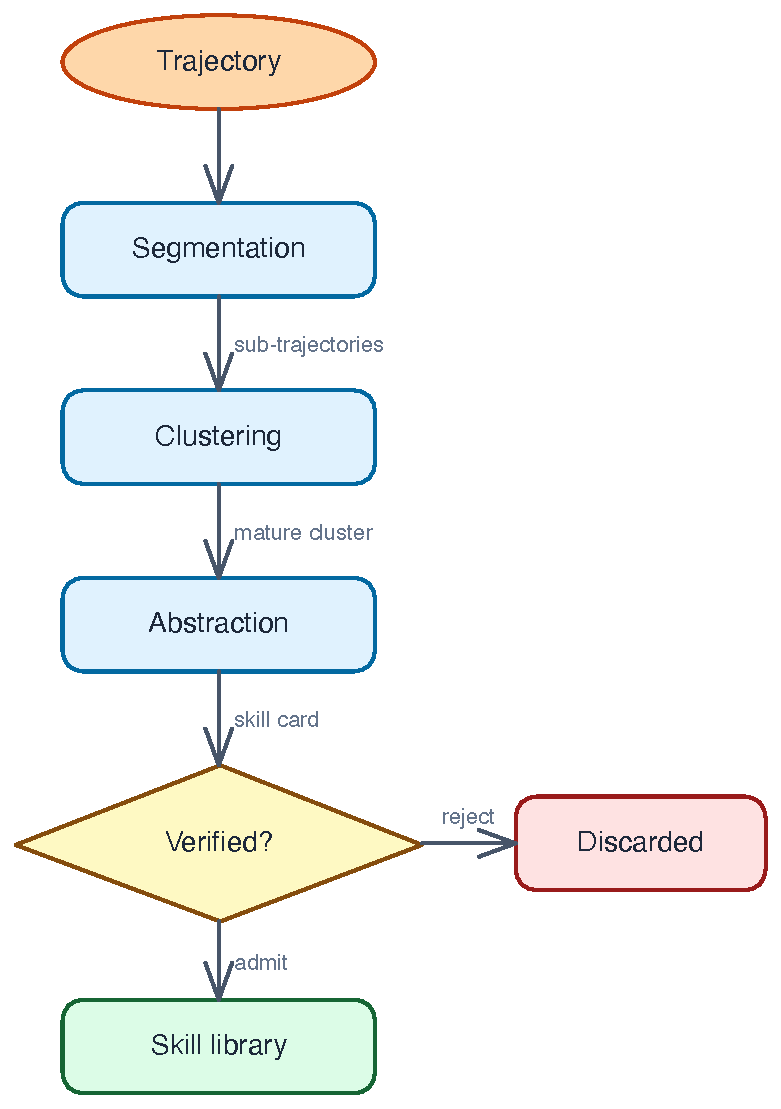
\includegraphics[width=0.48\textwidth]{Figures/fig_discovery.pdf}
\caption[The skill discovery pipeline]{The skill discovery pipeline. A
completed trajectory is segmented into sub-trajectories, streamed into
clusters, abstracted into a skill card, and admitted to the library only if
it passes verification; otherwise it is discarded.}
\label{fig:discovery}
\end{figure}

\subsection{Segmentation}

A trajectory typically interleaves several distinct behaviors (search, then
filter, then open a result). Segmentation cuts it into coherent
\emph{sub-trajectories}. Candidate cut points are seeded by two signals: URL
changes and drops in similarity between consecutive accessibility trees ---
the latter catches in-page transitions, such as a modal dialog opening, that
never touch the URL. An LLM then arbitrates the candidates, merging or
confirming cuts; its output is validated against the candidate set, and
trivial one-step navigation segments are merged into a neighbor.

\subsection{Streaming clustering}

Each sub-trajectory is embedded (using a sentence-encoder
representation~\cite{reimers2019sbert}) and assigned to a cluster by a
streaming, nonparametric clusterer in the DP-means
family~\cite{kulis2012dpmeans}: an incoming segment joins the nearest cluster
if its cosine similarity exceeds a threshold, and founds a new cluster
otherwise. The number of skills is therefore not fixed in advance, and
clustering happens online, during exploration, rather than in a separate
batch phase.

\subsection{Abstraction}

When a cluster matures --- it has recurred a configurable number of
independent times --- an LLM abstracts it into a \emph{skill card}: a name, a
description, and typed parameter slots that generalize over the concrete
values seen in the members (for example, the particular search string). The
member segments are retained as grounding evidence.

\subsection{Verification}

Following principle P1, a skill is admitted to the library only after
verification. In the deterministic mock environment used for development,
verification executes the skill in $k$ held-out contexts and requires every
run to succeed. On live websites, where re-execution is expensive and has
side effects, admission instead relies on recurrence across independent
trajectories (the maturity threshold) combined with outcome checks on the
episodes involved; Chapter~\ref{ch:discussion} discusses this trade-off.

\section{Semantic Task Generation via Operator Chaining}
\label{sec:method-semantic}

This section describes the centerpiece of the method: how the graph turns
verified skills into new, long-horizon training tasks that no single page
proposal would produce (Figure~\ref{fig:semantic}).

\begin{figure}[htbp]
\centering
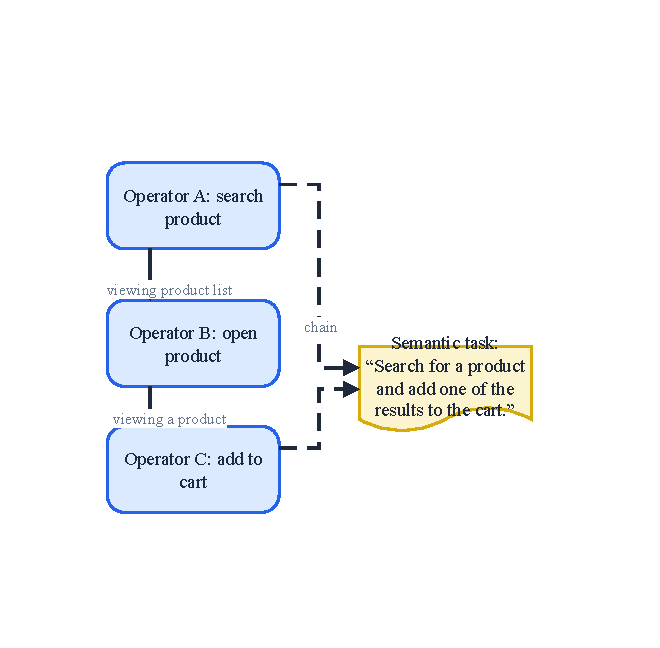
\includegraphics[width=0.78\textwidth]{Figures/fig_semantic.pdf}
\caption[Semantic task generation via operator chaining]{Semantic task
generation by operator chaining. Each edge is labelled with the shared state
where one operator's effect matches the next operator's precondition; chaining
the operators yields a single long-horizon semantic task that no individual
page proposes.}
\label{fig:semantic}
\end{figure}

\subsection{Operator induction}

When a skill is admitted, an LLM \emph{inducer} examines its skill card
together with the boundary observations (the pages before and after) of a few
member segments, and authors the skill's preconditions and effects as
natural-language predicates. Free-form authoring alone, however, fragments
the vocabulary: measured on a production run, embedding similarity failed to
unify a true paraphrase pair (scoring 0.570, below the merge threshold of
0.6) while scoring a false pair higher (0.606). Induction is therefore
\emph{vocabulary-aware}: the prompt includes the registry's existing
predicate labels --- the most frequent and most recent entries --- with an
instruction to reuse an equivalent predicate's exact text verbatim rather
than rephrase it.

Induced operators pass through an \emph{anti-tautology gate}. Any effect that
merely restates a precondition is dropped ($\mathit{eff} \leftarrow
\mathit{eff} \setminus \mathit{pre}$); a skill left with no novel effect is
rejected outright rather than promoted. This gate exists because, without it,
a majority of induced operators in early runs encoded no state change at all
--- and an operator that changes nothing can never chain toward anything new.
An operator is marked \emph{terminal} if one of its member episodes actually
reached a configured goal state, or if the inducer flags it as
goal-completing.

\subsection{Predicate canonicalization}

Each authored predicate is resolved against a \emph{predicate registry},
which reuses the same cosine-threshold clustering as the skill library but
with merging disabled, so identifiers stay stable once assigned: a new
predicate either joins an existing canonical cluster (and adopts its
identifier) or founds a new one. Operators thus share a common, growing
vocabulary $P = \{p_0, p_1, \dots\}$, and the planner can match effects to
preconditions by identifier equality --- keeping classical set-based planning
intact over an open, LLM-authored vocabulary.

\subsection{Chaining operators into semantic tasks}

The operator graph connects $\omega_1 \rightarrow \omega_2$ whenever an
effect of $\omega_1$ canonically matches a precondition of $\omega_2$. A
bounded depth-first enumeration lists all simple chains of length at least
two (with circuit breakers on path length and path count, since simple-path
enumeration is combinatorial in dense graphs). Each distinct chain becomes
one composed \emph{goal task}: its instruction is generated from the chained
skills' descriptions, and its starting point is the initiation URL recorded
for the first operator. For example, if exploration separately discovered
``search the product catalog'' and ``add a listed product to the cart'', the
chain of the two yields a task of the form \emph{``search for a product and
add one of the results to the cart''} --- a goal grounded in verified
capabilities, but never proposed by any single page.

Semantic tasks are scheduled conservatively: each distinct chain is attempted
once per run, and at most a fixed number of new chains is attempted per
visited node. Verification is deterministic when it can be: if the chain's
last operator is terminal and the site has a configured terminal predicate
(such as an order-confirmation URL), success is checked programmatically.
Otherwise the episode is self-graded through the solver's terminal answer and
then re-checked offline by the judge (Section~\ref{sec:method-data}). When
the graph is still too shallow to chain --- fewer than two connected
operators --- the system falls back to planning directly toward the terminal
predicate where one exists, so goal-directed data collection begins before
the graph has matured.

Semantic tasks matter for the end goal --- training data --- in two ways.
They extend the \emph{length distribution} of collected trajectories beyond
what single-page tasks produce, and they carry compositional structure: the
episode demonstrably strings multiple verified capabilities together, which
is precisely the behavior a small model most needs demonstrations of.

\section{Data Curation}
\label{sec:method-data}

Raw episodes are not yet training data. Three offline stages turn them into a
dataset while enforcing principle P1 end to end (Figure~\ref{fig:curation}).

\begin{figure}[htbp]
\centering
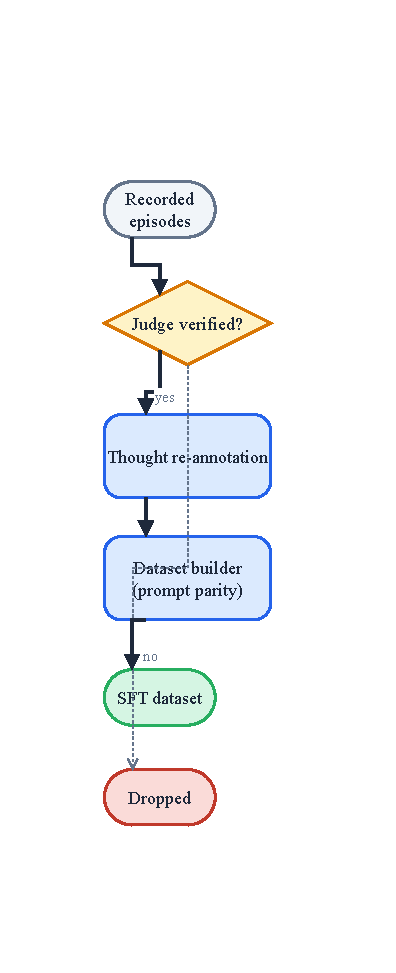
\includegraphics[width=0.50\textwidth]{Figures/fig_curation.pdf}
\caption[The data curation pipeline]{The data curation pipeline. Recorded
episodes are re-checked by an independent judge, their thoughts re-annotated,
and compiled by a prompt-parity dataset builder; declared successes that fail
judging are dropped.}
\label{fig:curation}
\end{figure}

\subsection{Independent judging of declared successes}

A solver that answers ``done'' has, in effect, graded its own homework. A
\emph{judge} pass re-examines every declared-success episode with a stronger
LLM, comparing the goal against the episode's own final state (URL and page
content), and records a verdict alongside the original outcome. The verdict
is additive --- original outcomes are never overwritten --- and the dataset
builder can be instructed to keep only judge-verified successes, dropping
never-judged episodes rather than silently trusting them.

\subsection{Thought re-annotation}

The solver's spontaneous thoughts are uneven in quality, and they are the
imitation target for the fine-tuned model. A re-annotation pass rewrites each
step's thought into a structured form composed of: a terse assessment of the
current state; a reflection when the previous action made no progress; the
step's current \emph{subgoal}, recovered by replaying the same segmentation
used during discovery over the recorded trajectory; and, only on a task's
final step, an explicit completion check against the goal. Crucially, the
subgoal appears only in the assistant \emph{target}, never in the user
prompt: at inference time no component exists to supply ``the current
subgoal'' as an input, and training must not assume one.

\subsection{Dataset construction with prompt parity}

The final builder compiles episodes into instruction-tuning examples under a
strict \emph{prompt parity} rule: the training-time prompt is byte-identical
in structure to the live solver's. The system prompt is imported from the
solver rather than duplicated; the page observation is capped by the same
truncation routine with the same explicit truncation marker; and history
lines are rendered with the same outcome annotations the live agent sees.
Steps whose recorded action failed to execute are excluded both as targets
and from later steps' history --- the error, after all, was never part of the
live agent's own history either. Episodes that ended in a justified
\texttt{report\_infeasible} are kept as valid targets. Each example carries
its trajectory identifier and step index, enabling trajectory-aware batching,
and examples are ordered easy-to-hard (shorter, verified episodes first) to
form a curriculum.

\section{Fine-Tuning the Small Language Model}
\label{sec:method-sft}

The target model is Qwen3.5-9B~\cite{yang2025qwen3}, fine-tuned with
LoRA~\cite{hu2022lora} using the LLaMA-Factory
framework~\cite{zheng2024llamafactory}. Two details are load-bearing. First,
the train/validation split is performed \emph{by trajectory}, never by step:
steps of one episode are strongly correlated, and splitting them across sets
would leak information. Second, the model family emits explicit reasoning
segments by default, while our targets are bare thought--action pairs; the
chat template must therefore disable the model's built-in ``thinking'' mode
consistently at training \emph{and} inference time. After training, the
adapter is merged and the model is served with vLLM~\cite{kwon2023vllm},
again with thinking disabled on every request, so the deployed model sees
exactly the distribution it was trained on --- the serving-side counterpart
of prompt parity.

\section{Implementation Notes}
\label{sec:method-impl}

HSGE is implemented in Python. Table~\ref{tab:modules} maps the pipeline
stages to modules. Two implementation decisions deserve mention. First, every
LLM-backed role --- explorer, solver, segmenter, abstractor, verifier,
inducer, judge, re-annotator --- is independently configurable, so cheap
models can serve high-volume roles while stronger models are reserved for
induction and judging. Second, the entire pipeline runs against deterministic
mock backends (a scripted LLM, a hash-based embedder, and a simulated
website) with no code changes: real backends are subclass swaps. This seam
makes the discovery logic unit-testable with exact assertions, and it
decouples algorithm development from API cost and website availability.
Artifacts (skills, operators, the graph, per-node results, and an event log)
are persisted after every explored node, so an interrupted run still leaves a
consistent snapshot.

\begin{table}[H]
\centering
\caption[Pipeline stages and implementation modules]{Pipeline stages and the
modules implementing them.}
\label{tab:modules}
\begin{tabular}{L{5.2cm} L{8.0cm}}
\toprule
\textbf{Stage} & \textbf{Module(s)} \\
\midrule
Exploration loop, frontier & \texttt{webarena/runtime}, \texttt{webarena/browser} \\
Task proposal and solving & \texttt{webarena/agents} \\
Segmentation & \texttt{segmentation}, \texttt{discovery} \\
Clustering, skill library & \texttt{clustering}, \texttt{abstraction}, \texttt{library} \\
Operators and planning & \texttt{operators}, \texttt{operator\_induction}, \texttt{predicate\_registry} \\
Data curation & \texttt{judge\_episodes}, \texttt{reannotate\_thoughts}, \texttt{build\_sft\_dataset} \\
Training and serving & LLaMA-Factory configs, vLLM scripts \\
\bottomrule
\end{tabular}
\end{table}

\vspace{1em}
\noindent
With the method in place, the next chapter turns to its empirical evaluation:
how much data the pipeline collects in practice, and whether fine-tuning on
that data improves a small model on the official WebArena benchmark.
